\chapter{Prototype 2}
\label{ch:prototype2}
Changes were made to the prototype based on the feedback and requirements that surfaced after the first focus group was conducted. This chapter details what changes were made and explains why they were necessary.

\section{Running prototype}
\label{sec:runningPrototype2}
Feedback from the first focus group was used to improve the visualizations, Table~\ref{fig:changeLog} shows a list of the changes made to the original system. U2, F2, T2 and T3 were discarded by the first focus group and were removed from the system for the second prototype. Requirement R1-8 was not implemented for prototype 2, beacuse there was not enough time to implement an entirely new concept (parsing two data sets and comparing them).

\begin{table}[h!]
  \centering
  \begin{tabular}{|l|l|l|p{8cm}|}
      \multicolumn{4}{c}{\textbf{Change log}} \\ \hline
      \textbf{Nr} & \textbf{ID} & \textbf{R1} & \textbf{Description} \\ \hline
      1  & U1  & 10       & Replaced smiley faces with coloured squares. \\ \hline
      2  & U1  & 1        & Classify using national/personal goals for sitting and walking.\\ \hline 
      3  & U2  &          & Removed. \\ \hline
      4  & F1  & 13, 14   & Added pictures to illustrate which activity each slice represents. \\ \hline
      5  & F1  &          & Removed nighttime from the dataset. \\ \hline
      6  & F2  &          & Removed. \\ \hline 
      7  & F3  & 10       & Changed sitting from red to white. \\ \hline
      8  & F3  &          & Removed nighttime from the dataset. \\ \hline
      10 & T1  & 6        & Added goal circles for each timeline. \\ \hline
      11 & T2  &          & Removed. \\ \hline
      12 & T3  &          & Removed. \\ \hline
      13 & T4  & 10       & Changed sitting colour to white. \\ \hline
      14 & T4  &          & Reduced inner radius of hour-ticks \\ \hline
      15 & All & 9        & Added option to switch between different colours including grayscale. \\ \hline
  \end{tabular}
  \caption{Changes made to the system after the first focus group.}
  \label{fig:changeLog}
\end{table}

% REVEIW
A new concept introduces after the first focus group was goals. Requirement R1-1 and R1-6 state that classifications should be based on goals and that some visualizations should display how the patients activity compares to the goals set. Two types of goals can be set: Time spent walking and time spent in an upright position. The first goal refers to \gls{ndh}'s recommendation of a minimum of 30 minutes activity each day, and 30 miutes are set as the default value for this goal. The second goal refers to the recommendation that an elderly person should be in a skeleton baring position for at lest 5 hours a day, to preserve the skeletal structure. 5 hours is the default value for the second goal.

New functionality added includes a new diagram T5, ability to set goals (default is national goals) and a small diagram, goal circles, that shows how active the patient was compared to the goals. The new diagram (see Figure~\ref{fig:t5}), T5, is similar to the visualization used by activPAL, but it does not show a bar for the amount of sedentary behaviour. The day is aggregated to 24 hour-blocks, the activity level for each hour is represented by stacked bars. This means that an hour with no activity, other than seating, will show no bar. 

Goal circles are small diagrams appended to T1 and T5, see Figure~\ref{fig:t1} and~\ref{fig:t5}. This was one of the new features in prototype 2 to satisfy requirement R1-6, which states that the users should be able to compare the patients activity to goals.  The circles are used to indicate how much activity the patient accumulated compared to the goals set. A full circle means the patient reached his goal that day. Exceeding the goal will produce additional circles. For example, if the goal was walking for 1 hour each day, a full circle would indicate that the patient walked exactly 1 hour, a half circle would indicate the patient walked 0.5 hours, and two circles would mean 2 hours of walking.

Table~\ref{tab:runProtDesc2} shows an overview of the visualizations included in the second version of the system. A functionality added to all the visualizations was the ability to switch between colours, including grayscale. The grayscale versions were used to create printouts for focus group 2, in accordance to requirement R1-9. U2 was discarded by the first focus group. U1, see Figure~\ref{fig:uSecond}, is the only overview chart available in the second prototype. The smilies were replaced with coloured squares because the sad face would be demotivating for the patients. U1 was also changed to classify the days compared to goals, as stated in requirement R1-1. The goals can be set manually, the default values are the national goals. Reaching both goals will classify the day to the green square, one goal to the yellow square, and no goals to the red square.

\begin{table}[h!]
  \centering
  \begin{tabular}{|c|p{11cm}|}
    \hline
    \textbf{ID} & \textbf{Description} \\ \hline
    U1 & Classifies each day of the week into either of three categories: Both goals reached, one goal reached and no goals reached. \\ \hline
    F1 & Pie chart showing the amount of activity for each day (Excluding what is assumed to be sleep during nighttime). \\ \hline
    F3 & Ball chart. Divides the pie slices of F1 into bubbles, each bubble representing one interval of activity (e.g. 2 hours of non-stop sedentary behaviour). \\ \hline
    T1 & Timeline of 24 squares, each square represents 1 hour of activity. The amount of activity in that hour is displayed using a gradient. \\ \hline
    T4 & One 24-hour clock showing the activity type using colour coding. \\ \hline
    T5 & Similar to T1, but instead of using a gradient the amount of activity is represented by stacked bars. \\ \hline
  \end{tabular}
  \caption{Visualizations included in prototype 2.}
  \label{tab:runProtDesc2}
\end{table}

\begin{figure}[h!]
  \centering
  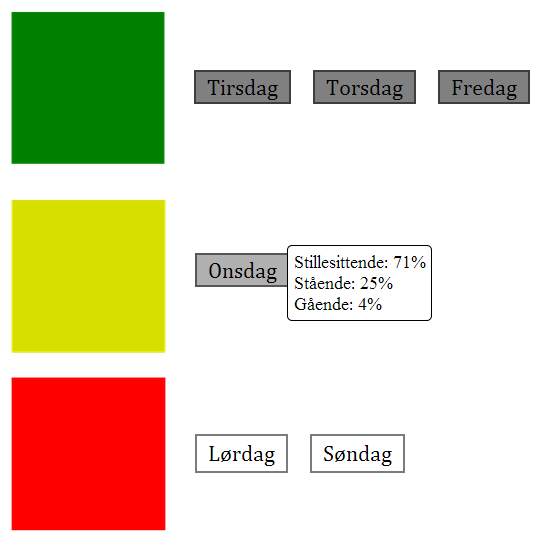
\includegraphics[width=0.5\textwidth]{u1Second.png}
  \caption[Second version of U1]{U1, the only overview chart in prototype 2.}
  \label{fig:uSecond}
\end{figure}

F2 was discarded and removed. The pictures from F2, illustrating the activity type, were added to the new version of F1, see Figure~\ref{fig:f1Second}. The feedback on F3 was less concise, in the first focus group the participants expressed some concern that all the red in the visualization would be demotivating for the patients. We therefore changed the colour of sedentary activity from red to white, as seen in Figure~\ref{fig.f3Second}. One of the comments from the first focus group regarding aggregated charts was that nighttime distorted the visualizations, nighttime was therefore removed from the data set for these charts in prototype 2.

\begin{figure}[h!]
  \centering
  \begin{subfigure}[b]{0.45\textwidth}
    \centering
    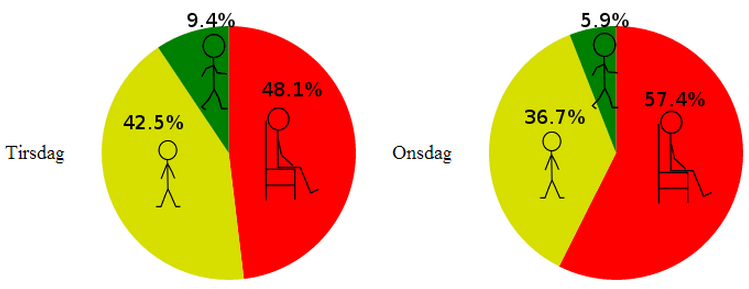
\includegraphics[width=\textwidth]{f1Second.png}
    \caption{F1}
    \label{fig:f1Second}
  \end{subfigure}
  \begin{subfigure}[b]{0.45\textwidth}
    \centering
    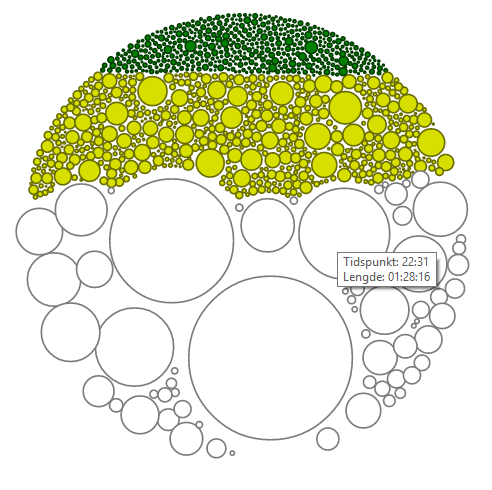
\includegraphics[width=\textwidth]{f3Second.png}
    \caption{F3}
    \label{fig:f3Second}
  \end{subfigure}
  \caption[Second version of F1 and F3]{Aggregated charts included in prototype 2.}
\end{figure}

T2 and T3 was discarded and removed. T1 was not changed other than the goal circle being appended to the right of each timeline, see Figure~\ref{fig:t1}. T4, see Figure~\ref{fig:t4}, received a colour change from red to white for sedentary activity, to further highlight actual activity. The inner radius of the hour-ticks, lines that marks each hour, was reduced to make the visualization look more like a normal clock. T5, see Figure~\ref{fig:t5}, was the only new visualization added. T5 uses stacked bars to show the activity level of each hour, and uses the goal circle to illustrate the patients activity compared to the goals set.

\begin{figure}[h!]
  \centering
  \begin{subfigure}[b]{0.6\textwidth}
    \centering
    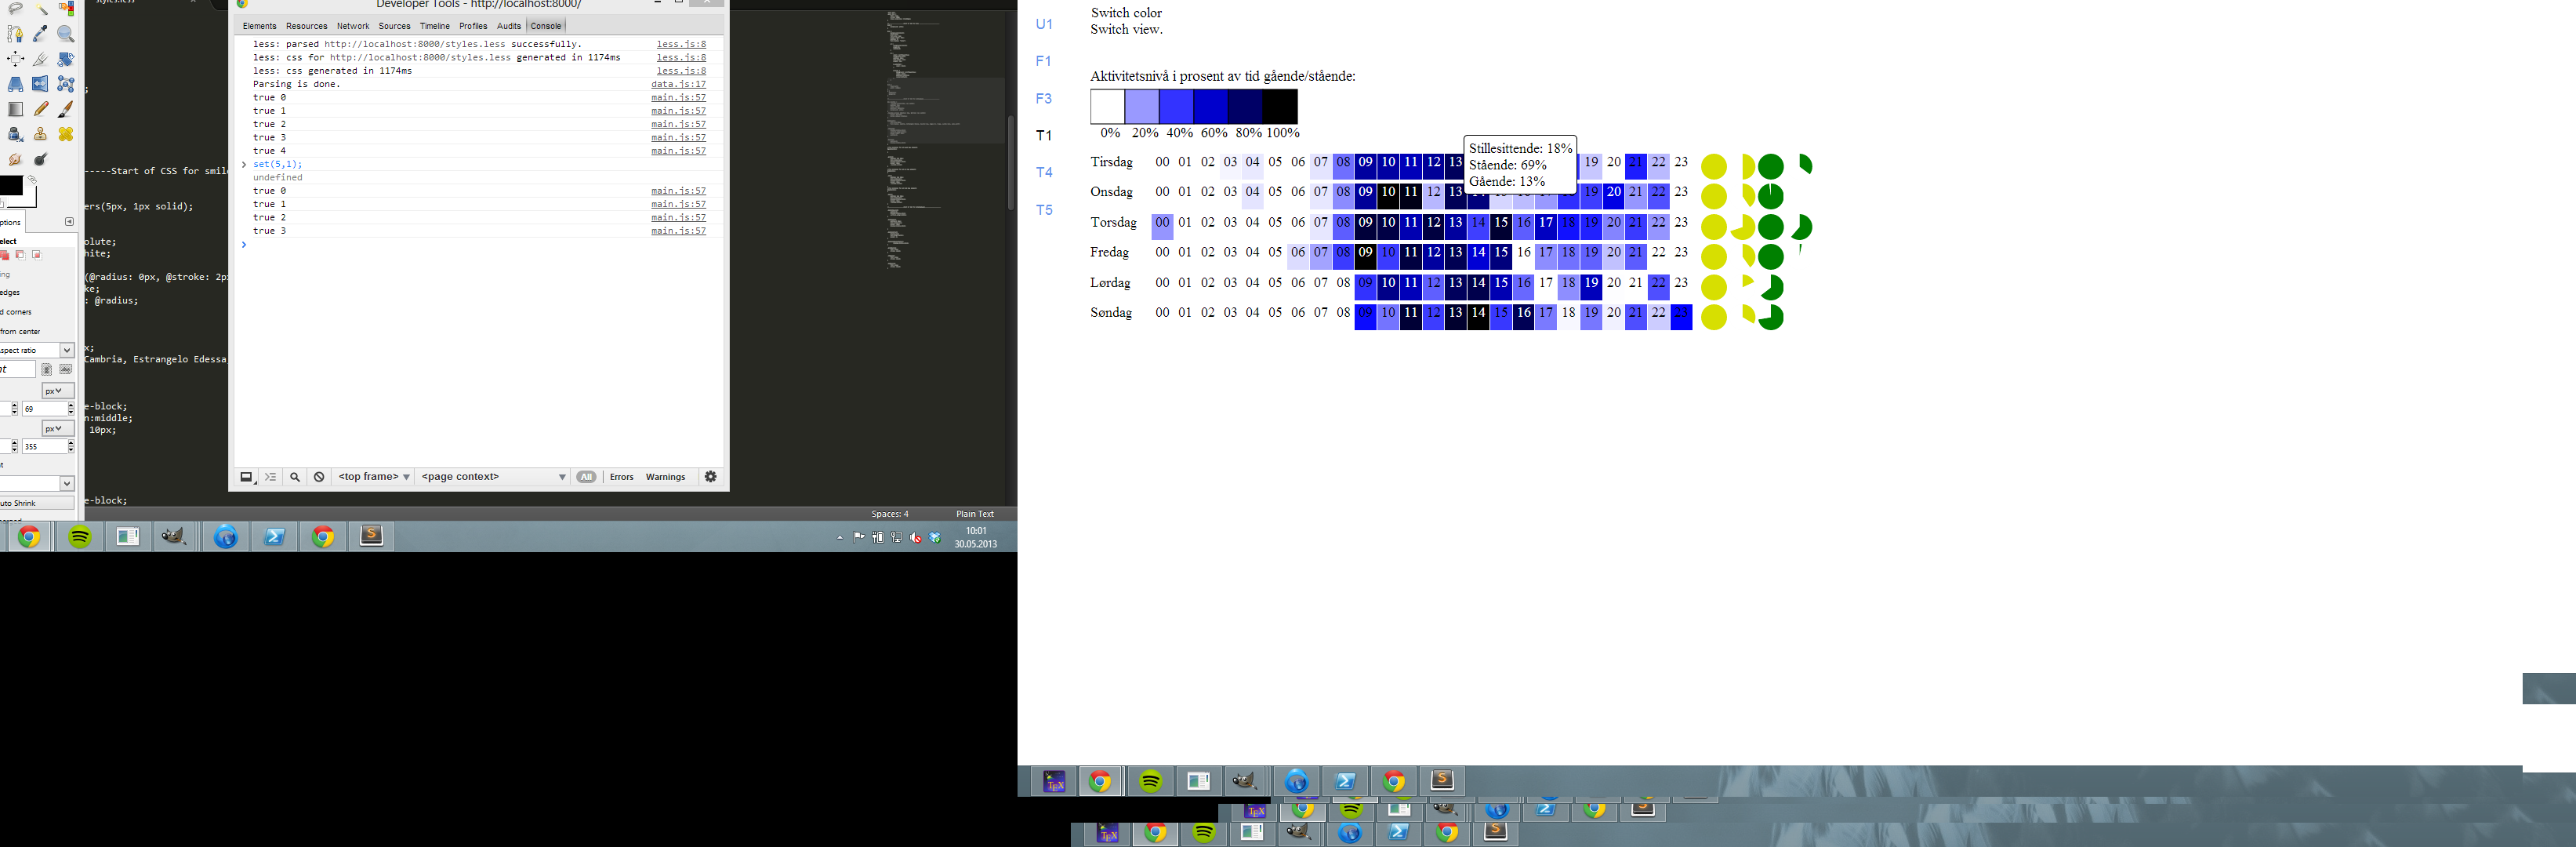
\includegraphics[width=\textwidth]{t1SecondWeek.png}
    \caption{T1}
    \label{fig:t1}
  \end{subfigure}
  \begin{subfigure}[b]{0.35\textwidth}
    \centering
    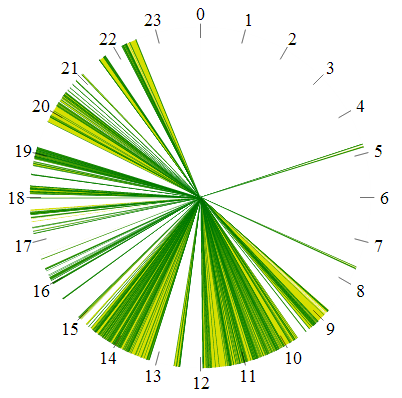
\includegraphics[width=\textwidth]{t4Second.png}
    \caption{T4}
    \label{fig:t4}
  \end{subfigure}
  \\
  \begin{subfigure}[b]{0.95\textwidth}
    \centering
    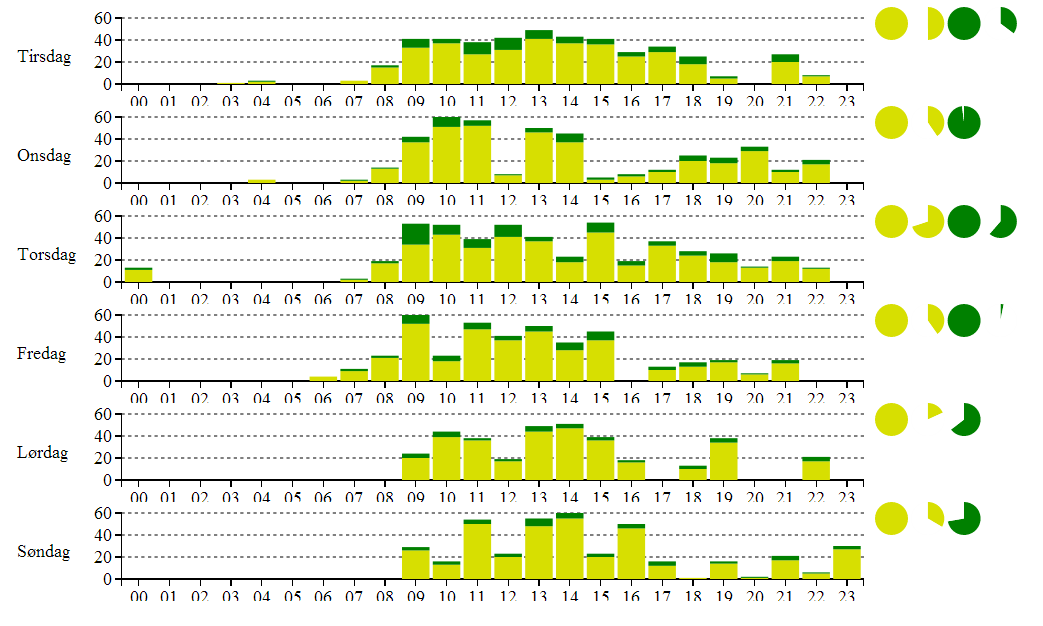
\includegraphics[width=\textwidth]{t5SecondWeek.png}
    \caption{T5}
    \label{fig:t5}
  \end{subfigure}
  \caption[Second version of T1, T4 and first version of T5]{Timeline charts included in prototype 2.}
\end{figure}
